\documentclass[a4paper, 10pt,onecolumn]{scrartcl}

%Standardpakete Deutsch
\usepackage[ngerman]{babel}
\usepackage[T1]{fontenc}
\usepackage[utf8]{inputenc}

%Extras
\usepackage{multirow}
\usepackage{natbib}
\usepackage{graphicx}
\usepackage{amsmath, amssymb}
\usepackage{graphicx}
\usepackage{grffile} %einfacheres einbinden von Dateipfaden
\usepackage{xpatch} %more space between title and subtitle
\usepackage{mathtools}
\usepackage{booktabs}
\newcommand{\changefont}[3]{
\fontfamily{#1} \fontseries{#2} \fontshape{#3} \selectfont}
\usepackage[export]{adjustbox}

\newlength{\myspace}
\setlength{\myspace}{2em}

\makeatletter
\xpatchcmd{\@maketitle}{\vskip.5em}{\vskip\myspace}{}{}
\makeatother

%\changefont{ptm}{m}{n}

\title{Computational Physics 1: Übung 7: Gewöhnliche Differentialgleichungen - Alpha-Verfahren} 
\author{Jakob Hollweck} %auch nach \begindocument möglich
\setlength{\parindent}{0pt}
\date{Abgabe 26.01.18}

\begin{document}
\maketitle


\section*{Aufgabe 1: Konvergenzverhalten des Alpha-Verfahrens}

In Abbildung \ref{Abbildung1} ist das Fehlerverhalten des $\alpha$-Verfahrens für verschiedene $\alpha$ dargestellt. Der Rückwärts-Euler mit $\alpha = 0$ ist ein rein implizites Verfahren und ist deswegen stabil, der Fehler divergiert nicht, sondern konvergiert in 1. Ordnung. Anzumerken ist, dass für kleine dt der globale Fehler linear mit 5dt zunimmt.
Das Crank-Nicolson-Verfahren für $\alpha = 0.5$ zeigt dagegen ein Fehlerverhalten 2. Ordnung mit dt, als einzige Konfiguration zeigt sie dies für alle dt. Die Konfigurationen mit $\alpha = 0.51$ und $\alpha = 0.501$ zeigen für große dt die gleiche Fehlerkonvergenz wie für $\alpha = 0.5$, für kleine dt hingegen ist der Fehler desto größer, desto weiter $\alpha$ entfernt von $\alpha = 0.5$ ist und nähert sich dem Fehler des Euler-Rückwärts-Verfahrens an. 
Betrachet man nun das Euler-Vorwärts-Verfahren, so ist gut zu erkennen, dass der Fehler mit hoher Ordnung divergiert. Wieder ist anzumerken, dass für kleine dt der globale Fehler linear mit 5dt zunimmt.

\begin{figure}[ht!]
	\centering
	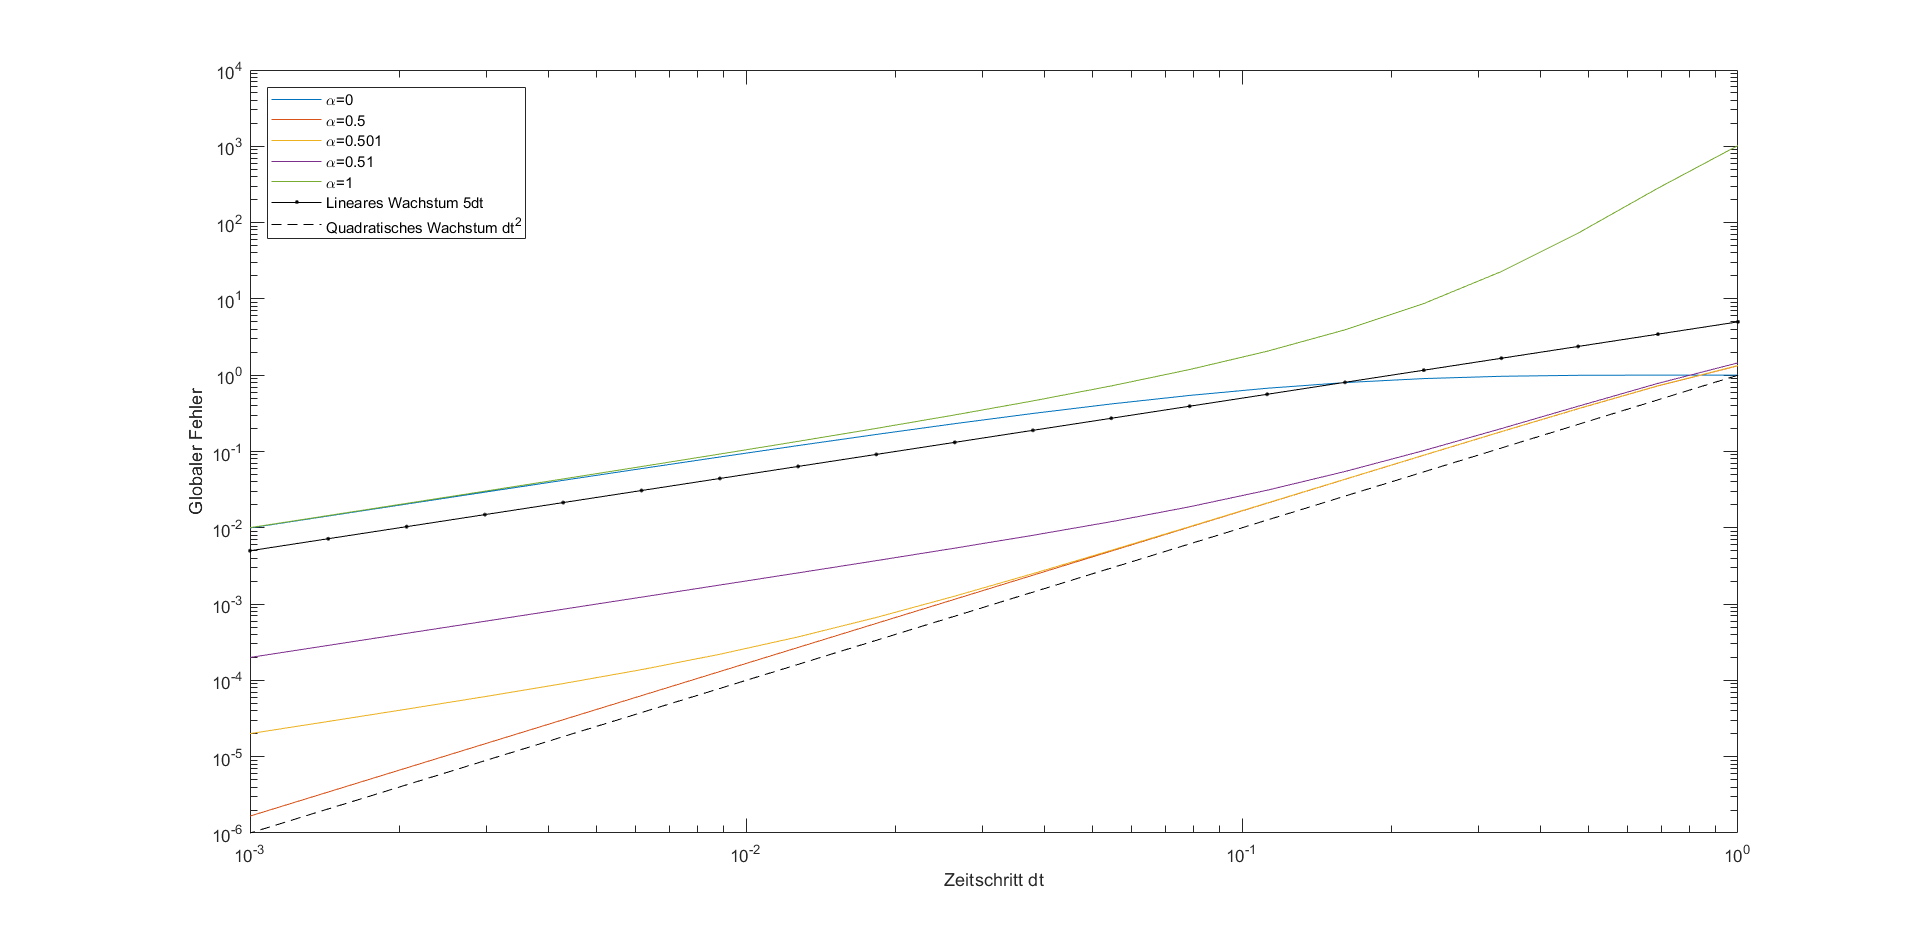
\includegraphics[scale=0.4,center]{Globaler Fehler_2.png}
	\caption{Der Globale Fehler verschiedener $\alpha$-Werte, aufgetragen über Zeitschritt dt. Zum Vergleich wurden die lineare Funktion $5$dt und die quadratische Funktion dt$^2$ eingefügt. } 
	\label{Abbildung1}
\end{figure}

\newpage

\section*{Aufgabe 2: Energie des harmonischen Oszillators}
 


\begin{figure}[ht!]
	%\centering
	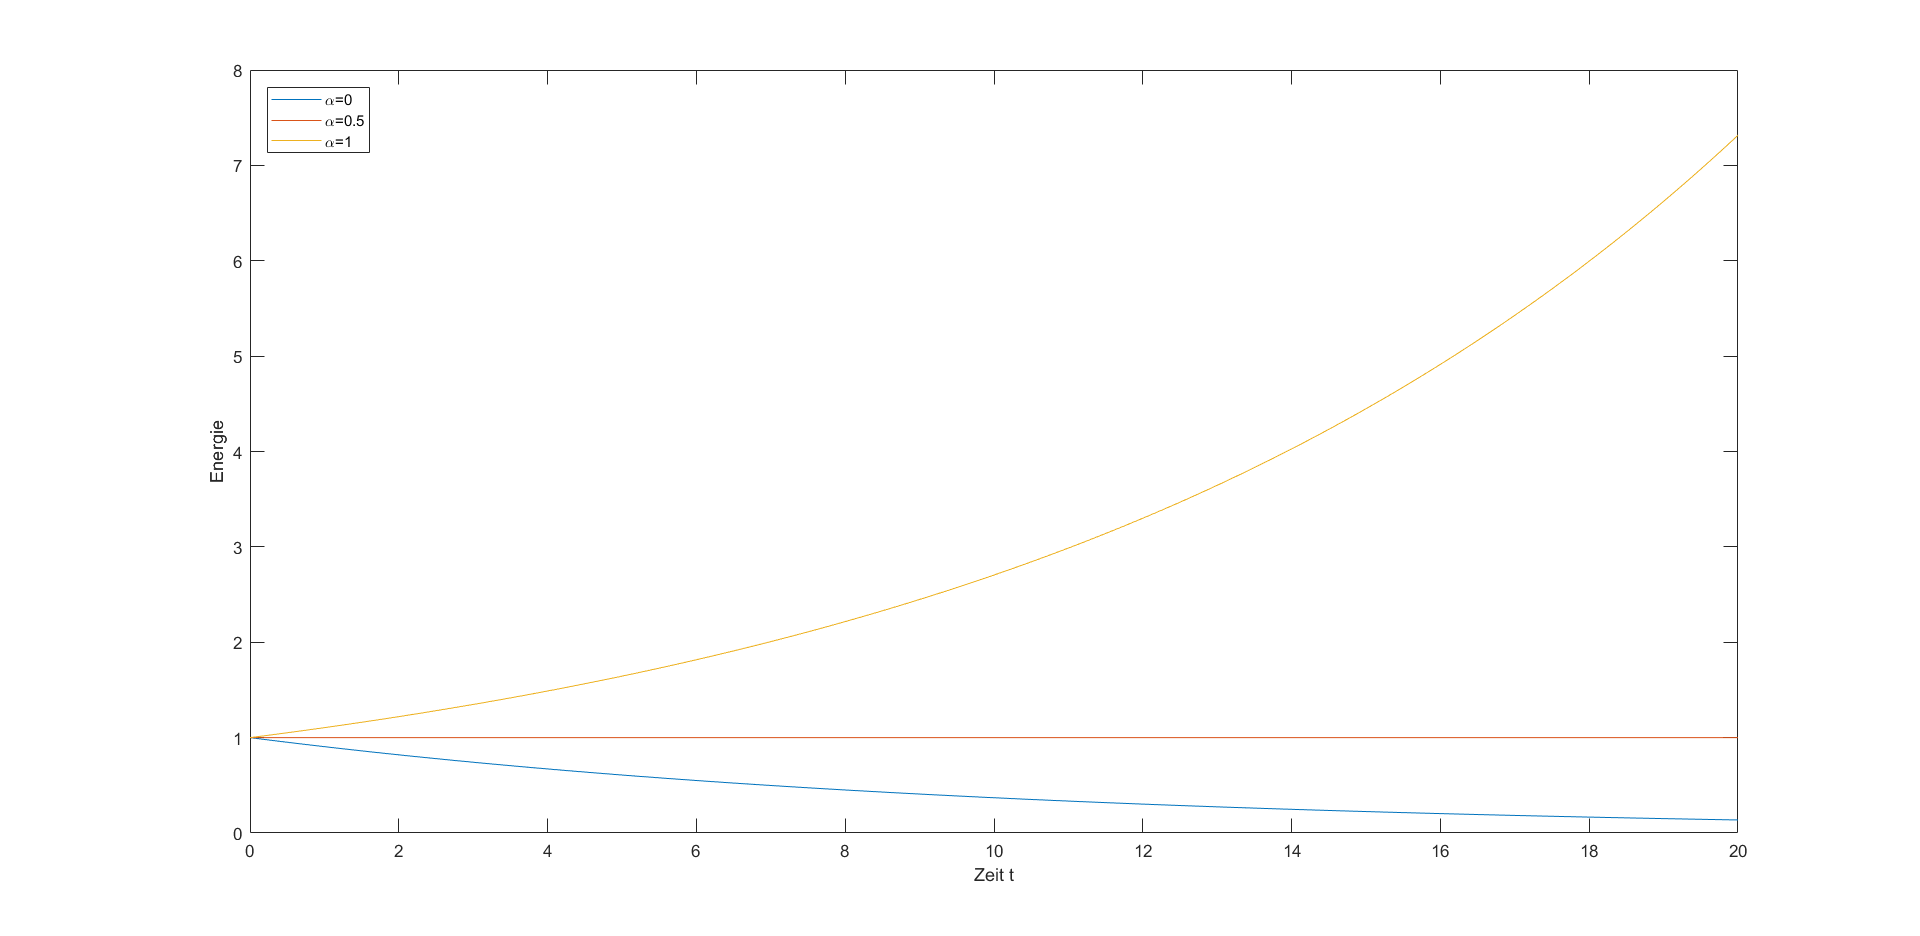
\includegraphics[scale=0.4,center]{Zeit_2.png}
	\caption{Verhalten der Energie des harmonischen Oszillators während der Integration mit dem Euler-Rückwärts- ($\alpha=0$), Crank-Nicholson- ($\alpha=0.5$) und Euler-Vorwärts-Verfahren ($\alpha=1$).} 
	\label{Abbildung2}
\end{figure}

In Abbildung \ref{Abbildung2} wurde das Verhalten der Energie des harmonischen Oszillators für verschiedene $\alpha$ untersucht. Für das Rückwärts-Euler-Verfahren ist zu erkennen, dass es sich bei diesem um ein implizites, also ein stabiles Verfahren handelt: Die Energie bleibt zwar nicht erhalten, scheint dafür aber gegen 0 zu konvergieren und divergiert nicht. Im Vergleich dazu ist das Euler-Vorwärts-Verfahren ein explizites Verfahren, es ist instabil, wodurch die Energie divergiert, die Energie bleibt also nicht erhalten. Dagegen ist das Crank-Nicolson-Verfahren gerade genau so beschaffen, dass sich die Abweichungen des Euler-Rückwärts- und Euler-Vorwärts-Verfahrens ausgleichen: Es ergibt sich ein gemischt explizit/implizites Verfahren, dass marginal stabil ist und in dem Falle des harmonischen Oszillators zu einer konstanten Energie, also zu Energieerhaltung führt. 

\end{document}